% Provenance (never printed): cycle 3 "La planete Terre. Les etres vivants
% dans leur environnement" (natural phenomena: volcanoes and earthquakes,
% natural hazards and the behaviour to adopt); see sources/book1/PROVENANCE.md.
% Book 1, grade 4, chapter 2.
\chapter{البراكين والزلازل: نظرة أولى}\label{ch:g4:volcanoes-earthquakes-first-look}

مساء الاثنين، تعرض نشرة الأخبار \omterm{def:g4:volcanoes-earthquakes-first-look:volcano}{بركانًا} في جزيرة بعيدة. وفي الظلام،
تتدفق نافورة من \omterm{def:g3:stones-pebbles-sand:rock}{صخر} برتقالي متوهج من شق في الأرض، وتنساب \omterm{def:g1:landscapes-around-us:water}{أنهار} من النار
ببطء على المنحدر حتى \omterm{def:g2:water-on-earth:ocean}{البحر}، وهي تفحّ ويتصاعد منها البخار. ويوم الخميس،
تعرض النشرة مكانًا آخر: بلدة صغيرة اهتزت فيها الأرض نصف دقيقة عند الفجر.
فسقطت المداخن في الشارع، وانزلق بيت قديم عن
أساسه.

حدثان مختلفان كل الاختلاف. لكن كليهما يأتي من أعماق الأرض، وكلاهما، كما
سنرى، يحدث في بعض مناطق العالم أكثر بكثير مما يحدث في
غيرها.

\begin{recall}
\omterm{def:g1:landscapes-around-us:landform}{الجبال} \omterm{def:g1:landscapes-around-us:landform}{والتلال} \omterm{def:g1:landscapes-around-us:landform}{والوديان} \omterm{def:g1:landscapes-around-us:landform}{والسهول} هي أشكال سطح الأرض
(\cref{ch:g1:landscapes-around-us}). واليابسة على الأرض مجموعة في سبع
\omterm{def:g3:continents-and-oceans:continent}{قارات}، بين خمسة محيطات؛ \omterm{def:g2:water-on-earth:ocean}{والمحيط} الهادئ أكبر المحيطات
(\cref{ch:g3:continents-and-oceans}).
\end{recall}

\section{بركان يثور}

في أعماق بعيدة تحت أقدامنا، باطن الأرض شديد الحرارة. وفي بعض الأماكن، يكون
\omterm{def:g3:stones-pebbles-sand:rock}{الصخر} هناك حارًا إلى حد أنه ينصهر. وهذا \omterm{def:g3:stones-pebbles-sand:rock}{الصخر} المنصهر أخف من \omterm{def:g3:stones-pebbles-sand:rock}{الصخر} الصلب
\omterm{def:g2:water-on-earth:ocean}{المحيط} به، فيصعد ببطء، كما تصعد السدادة في الماء. وحيث يجد منفذًا إلى
السطح، يولد \omterm{def:g4:volcanoes-earthquakes-first-look:volcano}{بركان}.

\begin{definition}[البركان]\label{def:g4:volcanoes-earthquakes-first-look:volcano}
\emph{البركان}\index{بركان} مكان يخرج فيه \omterm{def:g3:stones-pebbles-sand:rock}{صخر} منصهر من أعماق الأرض إلى
السطح، وهو أيضًا \omterm{def:g1:landscapes-around-us:landform}{التلة} أو \omterm{def:g1:landscapes-around-us:landform}{الجبل} الذي يبنيه \omterm{def:g3:stones-pebbles-sand:rock}{الصخر} المنصهر هناك، طبقة بعد
طبقة.
\end{definition}

\begin{definition}[الثوران والحمم والرماد البركاني]\label{def:g4:volcanoes-earthquakes-first-look:eruption}
\emph{الثوران}\index{ثوران} هو الوقت الذي يقذف فيه \omterm{def:g4:volcanoes-earthquakes-first-look:volcano}{البركان} \omterm{def:g3:stones-pebbles-sand:rock}{صخرًا} منصهرًا
ورمادًا وغازًا. و\emph{الحمم}\index{حمم} \omterm{def:g3:stones-pebbles-sand:rock}{صخر} منصهر ينسكب على السطح؛
فيسيل، ثم يبرد ويتصلب \omterm{def:g3:stones-pebbles-sand:rock}{صخرًا} جديدًا.
و\emph{الرماد البركاني}\index{رماد بركاني} قطع صغيرة جدًا من \omterm{def:g3:stones-pebbles-sand:rock}{الصخر} والزجاج
يقذفها الثوران في الهواء؛ ثم تتساقط كأنها \omterm{def:g4:clouds-rain-snow:precipitation}{ثلج} رمادي.
\end{definition}

\begin{omfigure}
\begin{tikzpicture}[font=\small]
  % ground and deep rock
  \fill[brown!30] (-5,-2.6) rectangle (5,0);
  % the volcano
  \fill[black!40] (-4.2,0) -- (-0.6,3.0) -- (0.6,3.0) -- (4.2,0) -- cycle;
  \fill[black!55] (-0.6,3.0) -- (-0.35,2.75) -- (0.35,2.75) -- (0.6,3.0) -- cycle;
  % layers inside the cone
  \foreach \k in {1,2,3}
    \draw[black!25] (-4.2+1.0*\k,0) -- (-0.6+0.05*\k,3.0-0.25*\k);
  % molten rock rising from deep below
  \fill[orange!80!red] (-0.25,-2.6) -- (-0.25,2.75) -- (0.25,2.75) -- (0.25,-2.6) -- cycle;
  \fill[orange!80!red] (0,-2.6) ellipse (1.6 and 0.5);
  % lava flow on the right flank
  \fill[orange!90!red] (0.5,2.9) .. controls (1.2,2.2) and (1.4,1.6) .. (2.2,1.0)
    .. controls (2.6,0.6) and (3.2,0.25) .. (3.7,0.1) -- (3.3,0.1)
    .. controls (2.6,0.35) and (2.0,0.75) .. (1.7,1.1)
    .. controls (1.2,1.6) and (0.9,2.3) .. (0.3,2.9) -- cycle;
  % ash and gas cloud
  \foreach \x/\y/\r in {0/3.6/0.45, -0.5/4.2/0.55, 0.4/4.3/0.5, -0.2/4.9/0.6, 0.6/5.0/0.55, -0.9/4.8/0.45, 0.1/5.5/0.6}
    \fill[black!25] (\x,\y) circle (\r);
  % labels
  \node[anchor=west] at (2.3,5.0) {رماد وغاز};
  \draw[black!60] (2.25,5.0) -- (1.1,4.9);
  \node[anchor=west] at (3.3,1.6) {سيل من الحمم};
  \draw[black!60] (3.25,1.6) -- (2.1,1.1);
  \node[anchor=east] at (-3.0,2.0) {البركان};
  \draw[black!60] (-2.95,2.0) -- (-1.9,1.5);
  \node[anchor=west, align=left] at (1.9,-1.4) {صخر منصهر يصعد\\من الأعماق};
  \draw[black!60] (1.85,-1.4) -- (0.3,-1.2);
\end{tikzpicture}

{\small \omterm{def:g4:volcanoes-earthquakes-first-look:volcano}{بركان} يثور (رسم، دون مراعاة النسب). يصعد \omterm{def:g3:stones-pebbles-sand:rock}{الصخر} المنصهر من الأعماق
ويخرج من القمة: فيسيل \omterm{def:g4:volcanoes-earthquakes-first-look:eruption}{حممًا} على المنحدر، بينما يُقذف الرماد والغاز عاليًا
في السماء. وكل \omterm{def:g4:volcanoes-earthquakes-first-look:eruption}{ثوران} يضيف طبقة جديدة إلى
\omterm{def:g1:landscapes-around-us:landform}{الجبل}.}
\label{fig:g4:volcanoes-earthquakes-first-look:volcano}
\end{omfigure}

ليست كل \omterm{def:g4:volcanoes-earthquakes-first-look:eruption}{الثورانات} متشابهة. ففي بعضها تكون \omterm{def:g4:volcanoes-earthquakes-first-look:eruption}{الحمم} سائلة: فتنسكب بهدوء أنهارًا
متوهجة قد تسيل كيلومترات، وتبلغ \omterm{def:g2:water-on-earth:ocean}{البحر} أحيانًا. وفي بعضها الآخر يكون \omterm{def:g3:stones-pebbles-sand:rock}{الصخر}
المنصهر لزجًا مليئًا بالغاز، كقارورة مشروب غازي رُجّت: فإذا انفجر خارجًا،
انفجر عمودًا هائلًا من الرماد يرتفع عاليًا في
السماء.

\begin{omfigure}
\begin{minipage}[b]{0.56\linewidth}\centering
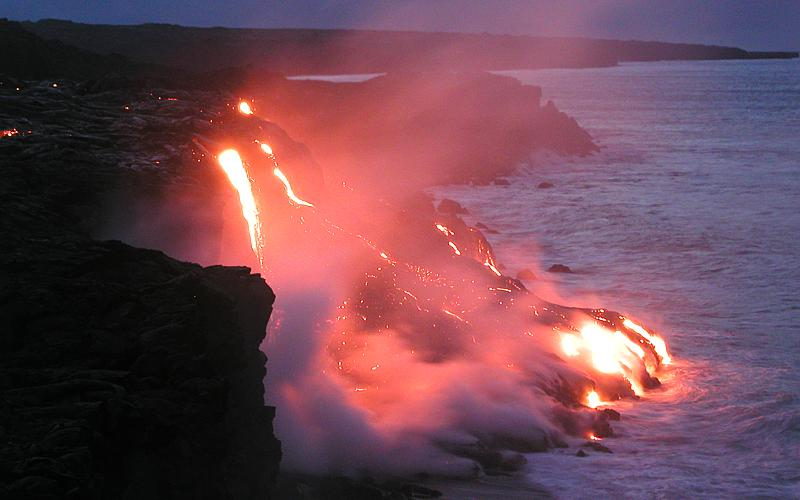
\includegraphics[width=\linewidth]{images/book1/g4-lava-ocean.jpg}

{\small \omterm{def:g4:volcanoes-earthquakes-first-look:eruption}{ثوران} سائل: \omterm{def:g4:volcanoes-earthquakes-first-look:eruption}{حمم} تنسكب من جرف بحري في \omterm{def:g2:water-on-earth:ocean}{المحيط}، في هاواي. الصورة:
مرصد هاواي \omterm{def:g4:volcanoes-earthquakes-first-look:volcano}{للبراكين} التابع لهيئة المسح الجيولوجي الأمريكية USGS (ملك عام).}
\end{minipage}\hfill
\begin{minipage}[b]{0.4\linewidth}\centering
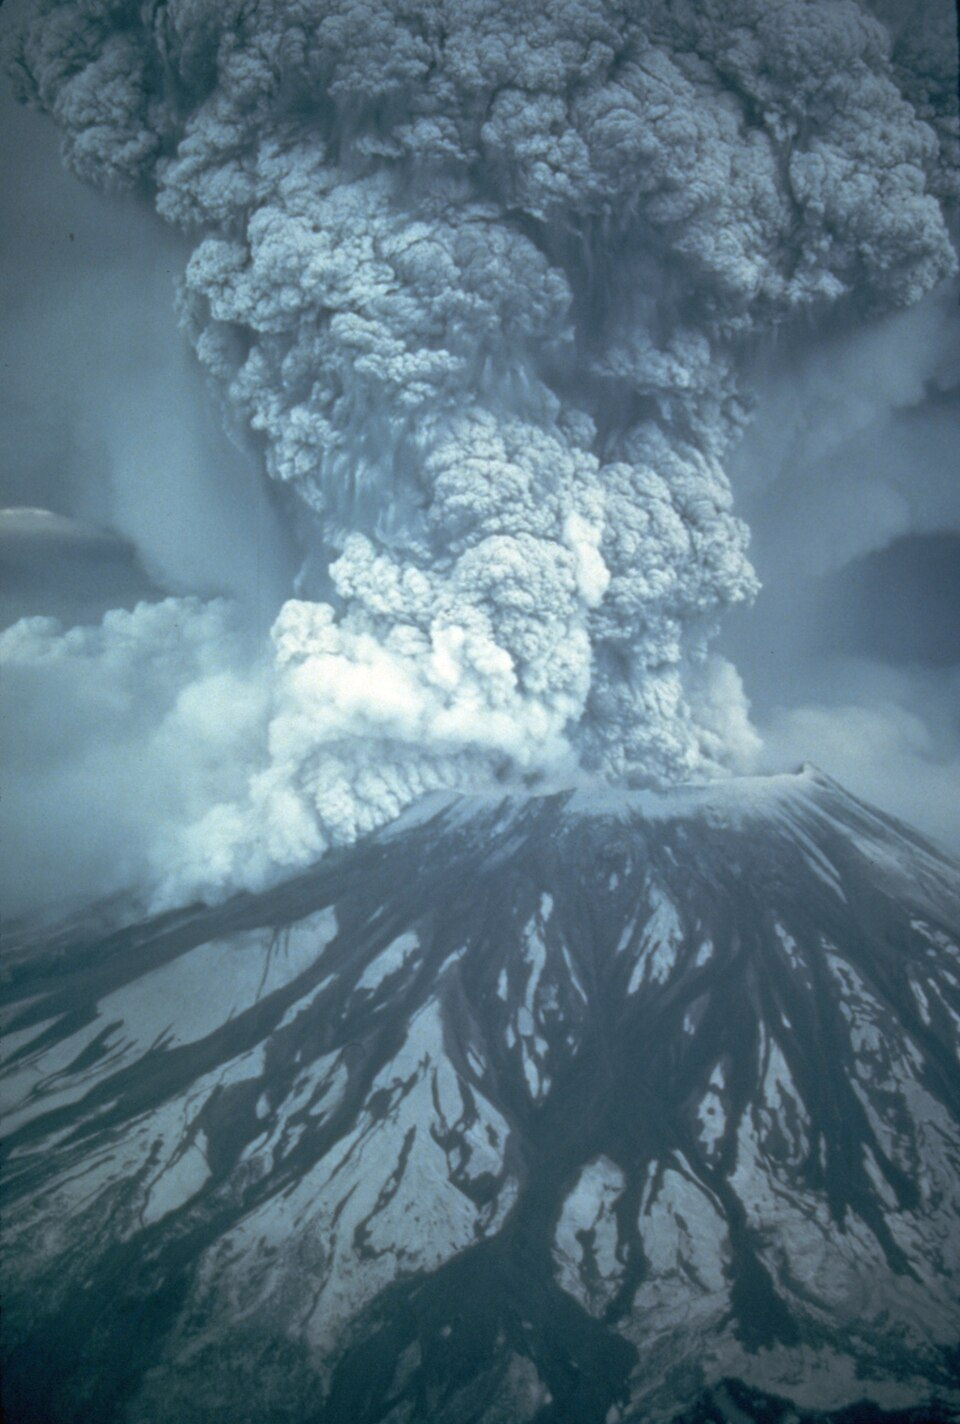
\includegraphics[width=0.78\linewidth]{images/book1/g4-st-helens.jpg}

{\small \omterm{def:g4:volcanoes-earthquakes-first-look:eruption}{ثوران} انفجاري: \omterm{def:g1:landscapes-around-us:landform}{جبل} سانت هيلينز، الولايات المتحدة، 18~مايو
1980. الصورة: أوستن بوست، USGS (ملك عام).}
\end{minipage}
% ledger: usgs:pu-oo-ocean, usgs:msh-1980
\label{fig:g4:volcanoes-earthquakes-first-look:two-eruptions}
\end{omfigure}

\begin{example}[جبل سانت هيلينز، 1980]\label{ex:g4:volcanoes-earthquakes-first-look:st-helens}
في ربيع عام 1980، نما انتفاخ على جانب \omterm{def:g1:landscapes-around-us:landform}{جبل} سانت هيلينز، إذ كان \omterm{def:g3:stones-pebbles-sand:rock}{الصخر}
المنصهر يندفع إلى الأعلى داخل \omterm{def:g1:landscapes-around-us:landform}{الجبل}. وفي صباح 18~مايو، هز \omterm{def:g4:volcanoes-earthquakes-first-look:earthquake}{زلزال} صغير
\omterm{def:g1:landscapes-around-us:landform}{الجبل}، فانزلق الانتفاخ في انهيار أرضي هائل، وانفجر \omterm{def:g4:volcanoes-earthquakes-first-look:volcano}{البركان} جانبيًا وإلى
الأعلى. واختفت أعلى 400~متر من \omterm{def:g1:landscapes-around-us:landform}{الجبل}: فصارت القمة فوهة
هائلة.
% ledger: usgs:msh-1980
\end{example}

\section{الأرض تهتز}

\omterm{def:g3:stones-pebbles-sand:rock}{الصخور} في الأعماق تحت أقدامنا ليست ساكنة تمامًا. فهي تُدفع وتُشد ببطء
شديد. وتنحني قليلًا، كمسطرة تضغط طرفيها --- حتى تنكسر فجأة وتنزلق.
فترسل الهزة الأرض مهتزة كيلومترات في كل
الاتجاهات.

\begin{definition}[الزلزال]\label{def:g4:volcanoes-earthquakes-first-look:earthquake}
\emph{الزلزال}\index{زلزال} اهتزاز مفاجئ للأرض، تسببه \omterm{def:g3:stones-pebbles-sand:rock}{صخور} تنكسر وتنزلق
في أعماق باطن الأرض.
\end{definition}

لا يدوم \omterm{def:g4:volcanoes-earthquakes-first-look:earthquake}{الزلزال} عادة إلا بضع ثوانٍ، وقد يدوم دقيقة أو دقيقتين في أكبرها.
وأكثر \omterm{def:g4:volcanoes-earthquakes-first-look:earthquake}{الزلازل} صغيرة إلى حد أن أحدًا لا يشعر بها: الأجهزة وحدها تلتقطها.
أما \omterm{def:g4:volcanoes-earthquakes-first-look:earthquake}{الزلزال} القوي فقد يجعل الأرض تتمايل كسطح سفينة، ويشق الطرق، ويهدم
الجدران والبيوت.

\begin{omfigure}
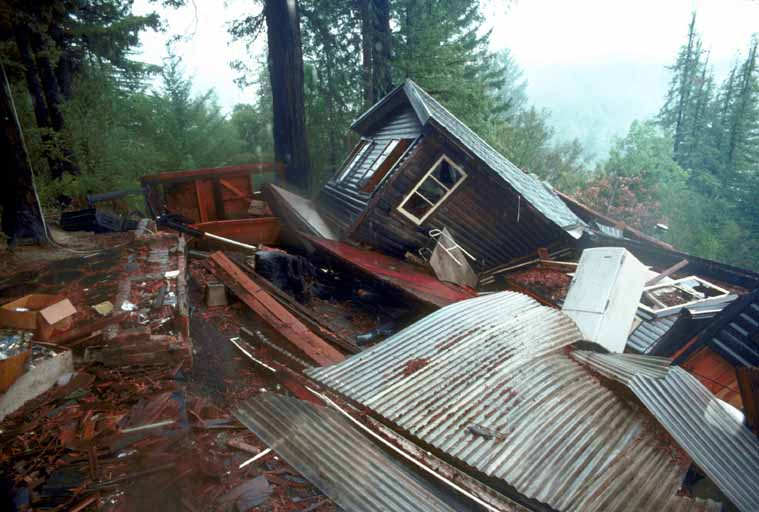
\includegraphics[width=0.55\linewidth]{images/book1/g4-loma-prieta-house.jpg}

{\small بعد \omterm{def:g4:volcanoes-earthquakes-first-look:earthquake}{زلزال} قوي في كاليفورنيا عام 1989: قُذف هذا البيت الخشبي جانبًا
عن أساسه الخرساني. الصورة: ج.~ك.~ناكاتا، USGS
(ملك عام).}
% ledger: usgs:loma-prieta-house
\end{omfigure}

\begin{remark}[كم مرة؟]\label{rem:g4:volcanoes-earthquakes-first-look:how-often}
يحتفظ الجيولوجيون بقائمة لكل \omterm{def:g4:volcanoes-earthquakes-first-look:earthquake}{الزلازل} الكبيرة على الأرض. وفي السنوات الخمسين
من 1976 إلى 2025، تعدّ القائمة 7\,031 \omterm{def:g4:volcanoes-earthquakes-first-look:earthquake}{زلزالًا} كبيرًا (قويًا بما يكفي
لإتلاف المباني القريبة منه): أي نحو 141 في السنة، أو قرابة 3 كل أسبوع.
أما أكبرها على الإطلاق، تلك التي قد تدمر مدنًا كاملة، فنحو 14 في السنة.
وعلى الأرض نفسها، ثار نحو 1\,200 \omterm{def:g4:volcanoes-earthquakes-first-look:volcano}{بركان} في آخر اثني عشر ألف
سنة تقريبًا.
% ledger: data:usgs-comcat, data:gvp
\end{remark}

\section{أين تحدث البراكين والزلازل}

لو حدثت \omterm{def:g4:volcanoes-earthquakes-first-look:volcano}{البراكين} \omterm{def:g4:volcanoes-earthquakes-first-look:earthquake}{والزلازل} في أي مكان كيفما اتفق، لتوزعت نقاطها على \omterm{def:g3:continents-and-oceans:world-map}{خريطة
العالم} توزعًا منتظمًا. لكنها ليست كذلك.

\omterm{def:g2:drawing-to-map:map}{الخريطة} أدناه تبين نمطًا لافتًا. فأكثر \omterm{def:g4:volcanoes-earthquakes-first-look:volcano}{البراكين} وأكثر \omterm{def:g4:volcanoes-earthquakes-first-look:earthquake}{الزلازل} الكبيرة تقع في
أحزمة طويلة ضيقة. وأطولها جميعًا يدور حول \omterm{def:g2:water-on-earth:ocean}{المحيط} الهادئ: من نيوزيلندا صعودًا
عبر إندونيسيا والفلبين واليابان، ثم إلى ألاسكا، ثم نزولًا على طول \omterm{def:g1:landscapes-around-us:water}{الساحل}
الغربي للأمريكتين حتى طرف تشيلي. ولكثرة براكينه، كثيرًا ما يسمى
«حزام النار».

\begin{example}[العدّ على الخريطة]\label{ex:g4:volcanoes-earthquakes-first-look:shares}
عددنا النقاط الواقعة في الحلقة المظللة (على بعد 500~كيلومتر أو أقل من
خطها الأوسط). فمن \omterm{def:g4:volcanoes-earthquakes-first-look:volcano}{البراكين} البالغ عددها 1\,214، يقع 837 في الحلقة: أي نحو 2
من كل 3. ومن \omterm{def:g4:volcanoes-earthquakes-first-look:earthquake}{الزلازل} الكبيرة جدًا البالغ عددها 696، يقع 532 في الحلقة: أي
نحو 3 من كل 4. والحلقة لا تغطي إلا جزءًا صغيرًا من الأرض، لكنها تضم أكثر
براكينها وزلازلها.
% ledger: data:gvp, data:usgs-comcat
\end{example}

\begin{omfigure}
\begin{tikzpicture}
\begin{axis}[ommap, width=\linewidth, xtick=\empty, ytick=\empty, grid=none,
    legend style={font=\scriptsize, at={(0.5,-0.02)}, anchor=north,
      draw=none, legend columns=3, /tikz/every even column/.append style={column sep=6pt}},
    legend cell align=left]
  \addplot[fill=omHypsLandA!85!black, draw=black!45, line width=0.2pt, forget plot]
    table {figdata/out/shared-geo-land.dat};
  \addplot[orange!80!black, opacity=0.35, line width=9pt, line cap=round, line join=round]
    table {figdata/out/grade-4-ring_of_fire-ring.dat};
  \addlegendentry{الحلقة حول المحيط الهادئ}
  \addplot[only marks, mark=triangle*, mark size=1.3pt, red!75!black]
    table[x=lon, y=lat] {figdata/out/grade-4-ring_of_fire-volcanoes.dat};
  \addlegendentry{\foreignlanguage{arabic}{بركان ثار في آخر \babelsublr{12\,000} سنة}}
  \addplot[only marks, mark=*, mark size=1.0pt, black, fill opacity=0.6]
    table[x=lon, y=lat] {figdata/out/grade-4-ring_of_fire-quakes7.dat};
  \addlegendentry{\foreignlanguage{arabic}{زلزال كبير جدًا بين \babelsublr{1976} و\babelsublr{2025}}}
\end{axis}
\end{tikzpicture}

{\small \omterm{def:g4:volcanoes-earthquakes-first-look:volcano}{البراكين} التي ثارت في آخر اثني عشر ألف سنة تقريبًا، وأكبر \omterm{def:g4:volcanoes-earthquakes-first-look:earthquake}{الزلازل}
في الفترة 1976--2025. أكثرها يقع على حلقة من سلاسل الجزر والسلاسل الجبلية حول
\omterm{def:g2:water-on-earth:ocean}{المحيط} الهادئ (المنطقة المظللة). البيانات: البرنامج العالمي \omterm{def:g4:volcanoes-earthquakes-first-look:volcano}{للبراكين} في
مؤسسة سميثسونيان؛ فهرس \omterm{def:g4:volcanoes-earthquakes-first-look:earthquake}{الزلازل} لهيئة المسح الجيولوجي الأمريكية؛ \omterm{def:g1:landscapes-around-us:water}{السواحل}
Natural Earth.}
\label{fig:g4:volcanoes-earthquakes-first-look:map}
% ledger: data:gvp, data:usgs-comcat, data:ne-land
\end{omfigure}

وهناك أحزمة أصغر: أحدها يعبر جنوب أوروبا وآسيا، من \omterm{def:g2:water-on-earth:ocean}{البحر} الأبيض المتوسط إلى
\omterm{def:g1:landscapes-around-us:landform}{جبال} الهيمالايا؛ وأحزمة أخرى تمتد في وسط المحيطات، حيث تختبئ \omterm{def:g4:volcanoes-earthquakes-first-look:volcano}{البراكين} تحت
الماء. وبعض الأماكن، مثل هاواي، فيها \omterm{def:g4:volcanoes-earthquakes-first-look:volcano}{براكين} بعيدة عن أي حزام. أما لماذا
تقع الأحزمة حيث تقع، فذلك سؤال يجيب عنه \cref{ch:g7:plate-tectonics}: والجواب يفسر شكل \omterm{def:g2:drawing-to-map:map}{الخريطة}
كلها.

\section{السلامة أولًا}

لا أحد يستطيع أن يوقف ثورانًا أو \omterm{def:g4:volcanoes-earthquakes-first-look:earthquake}{زلزالًا}. لكن معرفة ما يجب فعله تنقذ
الأرواح.

\begin{omfigure}
\begin{tikzpicture}[font=\small, line cap=round, line join=round]
  % --- panel 1: DROP onto hands and knees
  \begin{scope}[xshift=8cm]
    \draw[black!30] (-0.2,0) -- (2.8,0);
    \fill[omDef] (0.62,0.98) circle (0.21);
    \draw[omDef, line width=2.2pt] (0.88,0.98) -- (2.0,0.95);
    \draw[omDef, line width=2pt] (0.95,0.96) -- (0.95,0.05);
    \draw[omDef, line width=2pt] (2.0,0.95) -- (1.98,0.08) -- (2.65,0.08);
    \node[font=\bfseries] at (1.3,-0.45) {انبطح};
    \node[font=\scriptsize, align=center] at (1.3,-0.95) {على يديك\\وركبتيك};
  \end{scope}
  % --- panel 2: COVER under a table
  \begin{scope}[xshift=4cm]
    \draw[black!30] (-0.2,0) -- (2.8,0);
    \fill[brown!60!black] (-0.1,1.45) rectangle (2.7,1.6);
    \draw[brown!60!black, line width=2pt] (0.1,1.45) -- (0.1,0) (2.5,1.45) -- (2.5,0);
    \fill[omDef] (0.75,0.95) circle (0.2);
    \draw[omDef, line width=2.2pt] (0.95,0.85) -- (1.95,0.8);
    \draw[omDef, line width=2pt] (1.9,0.8) -- (1.65,0.05) -- (2.25,0.05);
    \draw[omDef, line width=2pt] (1.0,0.85) -- (0.7,1.2) -- (0.5,0.95);
    \node[font=\bfseries] at (1.3,-0.45) {احتمِ};
    \node[font=\scriptsize, align=center] at (1.3,-0.95) {غطِّ رأسك وعنقك\\تحت طاولة متينة};
  \end{scope}
  % --- panel 3: HOLD ON to the table leg
  \begin{scope}
    \draw[black!30] (-0.2,0) -- (2.8,0);
    \fill[brown!60!black] (-0.1,1.45) rectangle (2.7,1.6);
    \draw[brown!60!black, line width=2pt] (0.1,1.45) -- (0.1,0) (2.5,1.45) -- (2.5,0);
    \fill[omDef] (0.75,0.95) circle (0.2);
    \draw[omDef, line width=2.2pt] (0.95,0.85) -- (1.95,0.8);
    \draw[omDef, line width=2pt] (1.9,0.8) -- (1.65,0.05) -- (2.25,0.05);
    \draw[omDef, line width=2pt] (1.0,0.85) -- (0.7,1.2) -- (0.5,0.95);
    \draw[omDef, line width=2pt] (1.0,0.8) -- (0.45,0.6) -- (0.12,0.65);
    \node[font=\bfseries] at (1.3,-0.45) {تمسّك};
    \node[font=\scriptsize, align=center] at (1.3,-0.95) {بالطاولة حتى\\يتوقف الاهتزاز};
  \end{scope}
\end{tikzpicture}

{\small ما تفعله ما إن تبدأ الأرض بالاهتزاز: انبطح، واحتمِ،
وتمسّك.}
\label{fig:g4:volcanoes-earthquakes-first-look:drop-cover}
% ledger: shakeout:dch
\end{omfigure}

\begin{safety}
\textbf{أثناء \omterm{def:g4:volcanoes-earthquakes-first-look:earthquake}{الزلزال}.} ما إن تشعر باهتزاز الأرض:
\textbf{انبطح} على يديك وركبتيك؛ و\textbf{احتمِ} بتغطية رأسك وعنقك
بذراعك، وازحف تحت طاولة أو مكتب متين إن وُجد قريبًا منك؛
و\textbf{تمسّك} به حتى يتوقف الاهتزاز. لا تركض إلى الخارج والأرض تهتز،
ولا تقف عند عتبة الباب: فالزجاج والأشياء المتساقطة هي الخطر الأكبر. وحين
يتوقف، غادر المبنى بهدوء، كما تتدرب في تمارين الإخلاء في
المدرسة.

\textbf{قرب \omterm{def:g4:volcanoes-earthquakes-first-look:volcano}{بركان}.} يراقب العلماء \omterm{def:g4:volcanoes-earthquakes-first-look:volcano}{البراكين} التي قد تستيقظ. فإذا حذّروا من
\omterm{def:g4:volcanoes-earthquakes-first-look:eruption}{ثوران} قادم، طلبت السلطات من الناس مغادرة المنطقة. فاتبع تعليماتها فورًا،
ولا تقترب أبدًا لتتفرج.
\end{safety}
% ledger: shakeout:dch

\begin{omfigure}

\includegraphics[width=0.55\linewidth]{images/book1/ai/g4-earthquake-drill.jpg}

{\small تمرين على \omterm{def:g4:volcanoes-earthquakes-first-look:earthquake}{الزلزال}: التلاميذ يتدربون على «انبطح، واحتمِ،
وتمسّك» تحت طاولاتهم.}
\end{omfigure}

\section{تمارين}

\begin{exercise}[$\star$]\label{exo:g4:volcanoes-earthquakes-first-look:1}
\omterm{def:g4:volcanoes-earthquakes-first-look:eruption}{حمم} أم رماد أم غاز؟ (أ) \omterm{def:g1:landscapes-around-us:water}{نهر} من \omterm{def:g3:stones-pebbles-sand:rock}{الصخر} المنصهر المتوهج يسيل على منحدر؛
(ب) قطع صغيرة جدًا من \omterm{def:g3:stones-pebbles-sand:rock}{الصخر} تُقذف في السماء، ثم تتساقط كأنها \omterm{def:g4:clouds-rain-snow:precipitation}{ثلج} رمادي؛
(ج) شيء لا يُرى يخرج من \omterm{def:g4:volcanoes-earthquakes-first-look:volcano}{البركان} مع الرماد.
\end{exercise}

\begin{exercise}[$\star$]\label{exo:g4:volcanoes-earthquakes-first-look:2}
ما \omterm{def:g4:volcanoes-earthquakes-first-look:earthquake}{الزلزال}؟ هل يدوم ساعات، أم ثواني؟
\end{exercise}

\begin{exercise}[$\star$]\label{exo:g4:volcanoes-earthquakes-first-look:3}
رتّب الخطوات الثلاث: تمسّك؛ انبطح؛ احتمِ.
\end{exercise}

\begin{exercise}[$\star$]\label{exo:g4:volcanoes-earthquakes-first-look:4}
في \omterm{def:g2:drawing-to-map:map}{الخريطة} في الصفحة~\pageref{fig:g4:volcanoes-earthquakes-first-look:map}، حول
أي \omterm{def:g2:water-on-earth:ocean}{محيط} تقع أكثر \omterm{def:g4:volcanoes-earthquakes-first-look:volcano}{البراكين}؟
\end{exercise}

\begin{exercise}[$\star$]\label{exo:g4:volcanoes-earthquakes-first-look:5}
صواب أم خطأ؟ (أ) أكثر \omterm{def:g4:volcanoes-earthquakes-first-look:earthquake}{الزلازل} أصغر من أن يُشعر بها. (ب) تبقى \omterm{def:g4:volcanoes-earthquakes-first-look:eruption}{الحمم}
سائلة إلى الأبد. (ج) حين تهتز الأرض، فالأسلم أن تركض
إلى الخارج.
\end{exercise}

\begin{exercise}[$\star$]\label{exo:g4:volcanoes-earthquakes-first-look:6}
انظر إلى رسم \omterm{def:g4:volcanoes-earthquakes-first-look:volcano}{البركان} في الصفحة~\pageref{fig:g4:volcanoes-earthquakes-first-look:volcano}.
من أين يأتي \omterm{def:g3:stones-pebbles-sand:rock}{الصخر} المنصهر؟ ومن أين يخرج؟
\end{exercise}

\begin{exercise}[$\star\star$]\label{exo:g4:volcanoes-earthquakes-first-look:7}
جد على \omterm{def:g2:drawing-to-map:map}{الخريطة}: (أ) بلدًا من بلدان الأمريكتين فيه \omterm{def:g4:volcanoes-earthquakes-first-look:volcano}{براكين} كثيرة على
طوله كله؛ (ب) مجموعة جزر في وسط \omterm{def:g2:water-on-earth:ocean}{المحيط} الهادئ،
فيها \omterm{def:g4:volcanoes-earthquakes-first-look:volcano}{براكين}، ولا تقع على الحلقة.
\end{exercise}

\begin{exercise}[$\star\star$]\label{exo:g4:volcanoes-earthquakes-first-look:8}
يحدث نحو 141 \omterm{def:g4:volcanoes-earthquakes-first-look:earthquake}{زلزالًا} كبيرًا في السنة. فكم \omterm{def:g4:volcanoes-earthquakes-first-look:earthquake}{زلزالًا} يقابل ذلك تقريبًا في
الشهر؟ (في السنة 12 شهرًا؛ أعطِ عددًا صحيحًا.)
\end{exercise}

\begin{exercise}[$\star\star$]\label{exo:g4:volcanoes-earthquakes-first-look:9}
نحو 3 من كل 4 \omterm{def:g4:volcanoes-earthquakes-first-look:earthquake}{زلازل} كبيرة جدًا تحدث في الحلقة حول \omterm{def:g2:water-on-earth:ocean}{المحيط} الهادئ. فمن
بين 20 \omterm{def:g4:volcanoes-earthquakes-first-look:earthquake}{زلزالًا} كبيرًا جدًا، كم \omterm{def:g4:volcanoes-earthquakes-first-look:earthquake}{زلزالًا} تتوقع تقريبًا في الحلقة؟ وكم
خارجها؟
\end{exercise}

\begin{exercise}[$\star\star$]\label{exo:g4:volcanoes-earthquakes-first-look:10}
أثناء تمرين على \omterm{def:g4:volcanoes-earthquakes-first-look:earthquake}{الزلزال}، ركض ليو ليقف عند باب الفصل. ماذا كان عليه أن
يفعل بدلًا من ذلك، ولماذا؟
\end{exercise}

\begin{exercise}[$\star\star\star$]\label{exo:g4:volcanoes-earthquakes-first-look:11}
من \omterm{def:g4:volcanoes-earthquakes-first-look:volcano}{البراكين} البالغ عددها 1\,214 على \omterm{def:g2:drawing-to-map:map}{الخريطة}، يقع 837 في الحلقة حول \omterm{def:g2:water-on-earth:ocean}{المحيط} الهادئ.
كم \omterm{def:g4:volcanoes-earthquakes-first-look:volcano}{بركانًا} يقع خارجها؟ وهل عبارة «نحو 2 من كل 3» طريقة جيدة لوصف
نصيب الحلقة؟ (تلميح: كم ثلثا 1\,200؟)
\end{exercise}
